\section{Event Selection}
\label{sec:EventSel}

A $ZZ^*(\rightarrow 4\ell) jj$ event at the detector-level consists of a lepton quadruplet formed by two SF-OC lepton pairs from each $Z$ boson decay and a dijet from the initial state partons. The quadruplet is formed in events with four prompt leptons (electrons or muons), where the leading and sub-leading leptons satisfy $p_{T} > 20$ GeV to ensure a high trigger efficiency. Due to momentum conservation, the prompt leptons are separated from each other. Therefore, all prompt leptons in an event must have $\Delta R > 0.05$ to reduce contributions from mis-reconstruction while keeping leptons from possible boosted production scenarios. Additionally, each SF-OC lepton pair's invariant mass is required to satisfy $m_{\ell \ell } > 5$ GeV to suppress the contamination from lower resonance backgrounds. A quadruplet is formed from the two SF-OC lepton pairs whose invariant masses are closest and next closest to the mass of the Z-boson ($m_{Z}$). Based on these requirements, the quadruplets can be of the following three types:

\begin{itemize}
\item{$4e$: events with two $e^{+}e^{-}$ pairs.}
\item{$4\mu$: events with two $\mu^{+}\mu^{-}$ pairs.}
\item{$2e2\mu$ or $2\mu2e$: events where one of the pair is $e^{+}e^{-}$ and other is $\mu^{+}\mu^{-}$}
\end{itemize}

Once the quadruplet is formed, the leading-lepton pair is defined as the one with a higher absolute rapidity value, i.e., $|y_{ij}|$. This additional identification is motivated by consistently defining the leading and sub-leading pairs at both particle and detector levels to reduce the resolution-induced bin migrations, which need to be corrected by the unfolding procedure. The quadruplets with all four leptons passing the signal lepton criteria of the TTVA and isolation are the \textit{signal quadruplet} defining the signal region. The quadruplets with one or more lepton failing either the isolation or TTVA requirement are the \textit{non-signal quadruplets} and are used in the non-prompt background estimation. The invariant mass of the quadruplet ($m_{4\ell}$) must be greater than 130 GeV to exclude the events from on-shell $H\rightarrow ZZ^*$ production, which are measured extensively by ATLAS analyses focused on Higgs measurements.

The final state jets in electroweak production of $ZZ^*(\rightarrow 4\ell) jj$ come from the initial state quarks on the opposite sides of the interaction point. Thus, the dijet is selected by requiring two signal jets defined in Section \ref{subsec:JetRecon} from the opposite side of the detector, i.e., $\eta_{leading~jet} \times \eta_{sub-leading~jet} < 0$. To maximize the probability of selecting an event from EWK $ZZ^*(\rightarrow 4\ell)jj$ production, a requirement of significant rapidity difference between the jets of $\Delta y_{jj}> 2 $ and a large invariant mass of $m_{jj} > 300 $ GeV are imposed on the dijet selection. 

\subsection{Signal Region}
\label{subsec:SignalRegion}
The two $Z$ bosons in the electroweak production of $ZZjj$ are produced centrally with respect to the dijet. Thus, the signal region of the analysis is defined based on the centrality ($\zeta$) of the di-$Z$boson production in an event. Centrality depends on the rapidity of the quadruplet and the rapidity of the dijet as:
\begin{equation}
    \zeta~=~\frac{|y_{quadruplet}~-~ 0.5*(y_{leading~jet}~+~y_{sub-leading~jet})| }{|y_{leading~jet}~-~y_{sub-leading~jet}|}
    \label{eq:centr}
\end{equation}

Figure \ref{fig:centrality_a} shows the predicted MC distribution of centrality for the three main production modes of $ZZ^*(\rightarrow 4 \ell)jj$. The significance of the EWK component over the inclusive parton initiated and $gg$-loop initiated QCD production is defined as, 
\begin{equation}
    s=\frac{N_{EWK}}{\sqrt{N_{QCD}^{(qq)}+N_{QCD}^{(gg)}}}
    \label{eqn:EWKSignificance}
\end{equation}
where $N_{EWK}$, $N_{QCD}^{(qq)}$ and $N_{QCD}^{(gg)}$ are the numbers of events from electroweak, parton-initiated QCD and gluon-loop initiated QCD productions, respectively. The chosen cut value on the centrality maximizes the EWK significance while maintaining a good selection efficiency of EWK events. Figure in \ref{fig:centrality_b} shows the efficiency and significance for various cut values of centrality.  

A VBS-Enhanced signal region is defined based on events with a quadruplet, a dijet, and $\zeta<0.4$. The low value of the centrality and the requirements for a signal dijet ensures that the events in this signal region originate in a more significant fraction from the electroweak production of $ZZ^*(\rightarrow 4 \ell) jj$. A VBS-Suppressed control region is also defined based on events with a quadruplet, a dijet, and $\zeta>0.4$. These events mainly originate from the QCD production of $ZZ^*(\rightarrow 4 \ell) jj$ and are used to optimize the analysis strategies. Table \ref{tab:EventSelection} summarizes all selections applied to select $ZZ^*(\rightarrow 4\ell)jj$ detector-level events.

\begin{figure}[!htbp]
\begin{subfigure}{.48\textwidth}
  \centering
  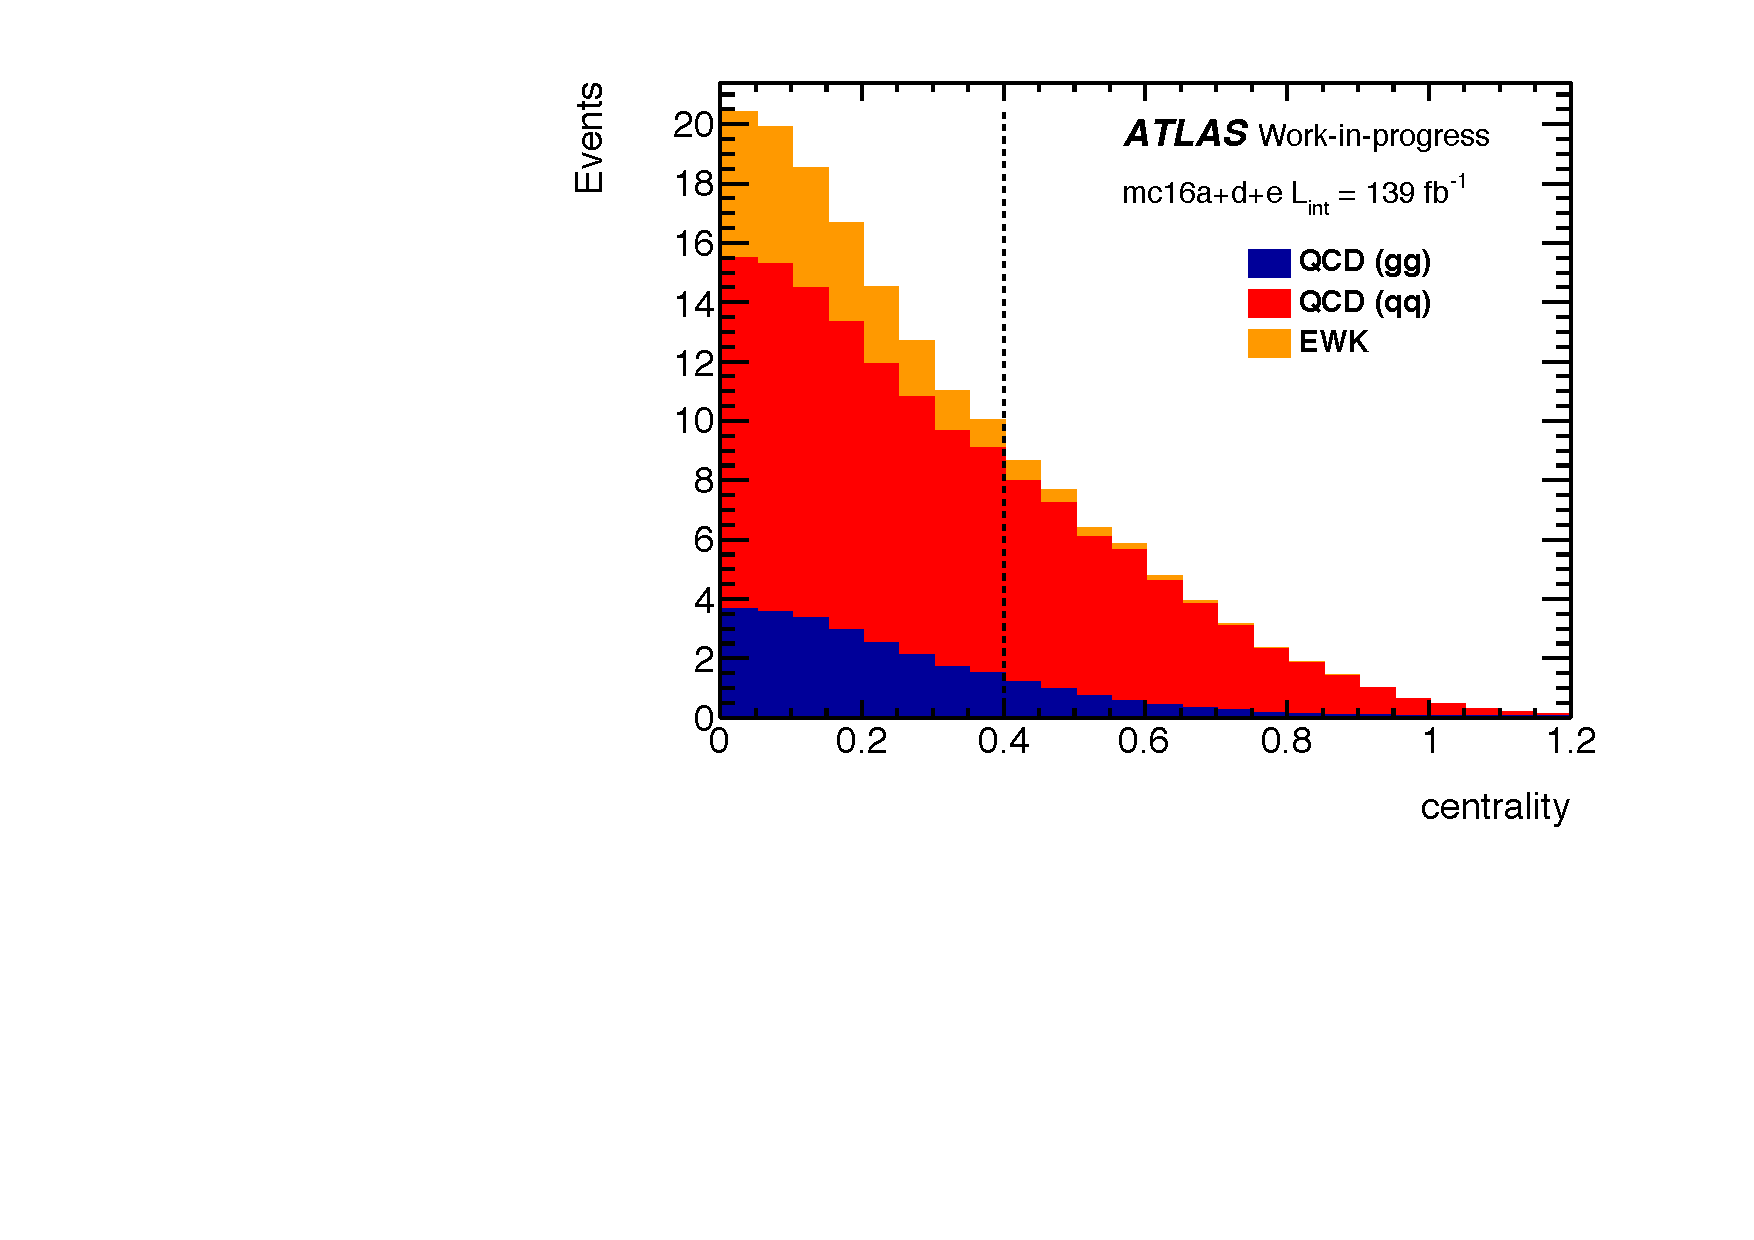
\includegraphics[width=.95\linewidth]{figures/AnalysisOverview/centrality_Dist.pdf}  
  \caption{Yields of EWK and QCD production.}
  \label{fig:centrality_a}
\end{subfigure}
\begin{subfigure}{.48\textwidth}
  \centering
  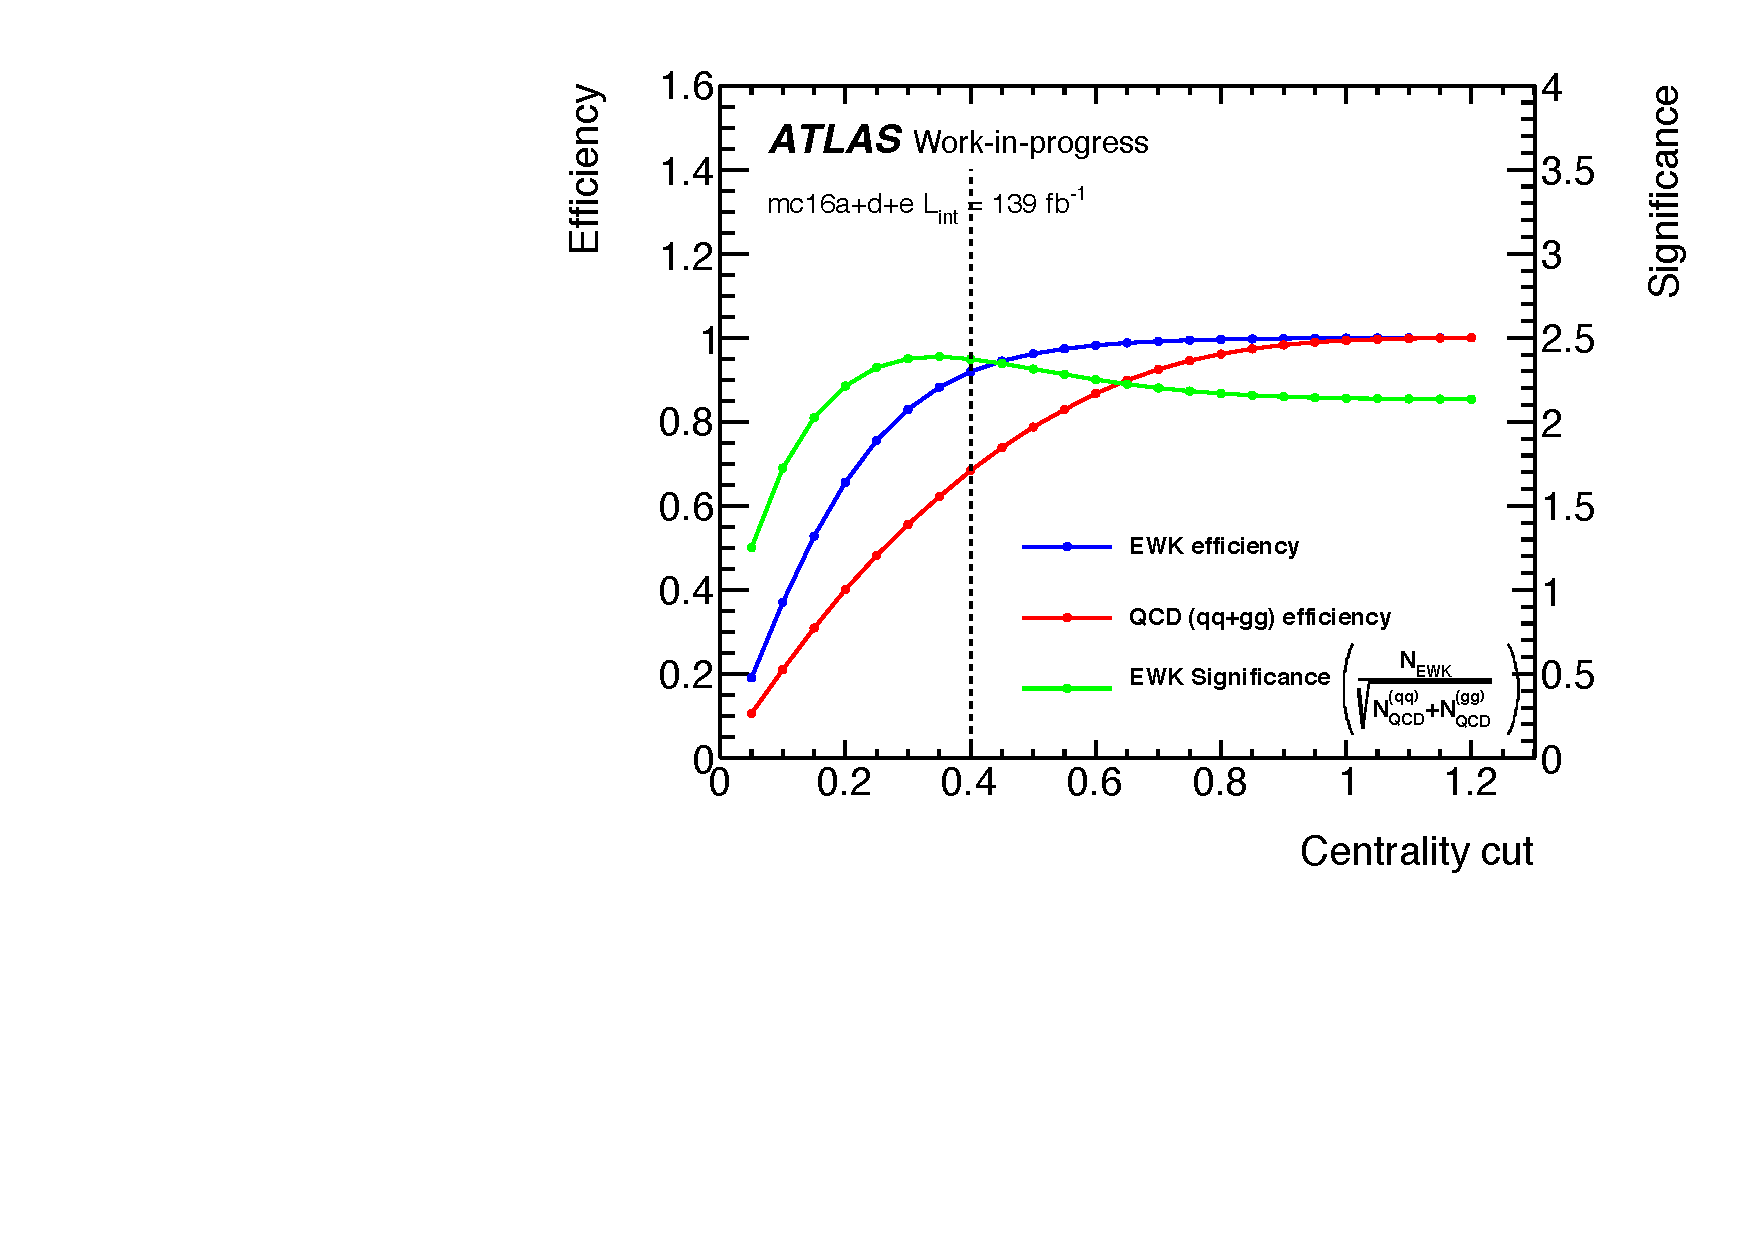
\includegraphics[width=.9\linewidth]{figures/AnalysisOverview/centrality_Cut.pdf}  \\
  \caption{Selection efficiency and EWK significance. }
  \label{fig:centrality_b}
\end{subfigure}
\caption{Centrality dependence for yield, EWK selection efficiency, and EWK significance. }
\end{figure}

\begin{table}[!htbp]
    \centering
        \caption{Details of event selection.\label{tab:EventSelection}}
        \begin{tabular}{|| l || c | c ||}
        \hline
        Event Selection         & Cut                   & Requirement                                                       \\
        \hline\hline
        Event               & Trigger                   &  Fire at least one lepton trigger                                     \\
        Preselection                & Vertex                    & At least one vertex with $2$ or more tracks                               \\
        \hline  
                    & Lepton Kinematics         & $p_{T} > 20$ GeV for two leading leptons                     \\
                    & Lepton Separation         & $\Delta R_{ij} > 0.05$ between leptons in quadruplet      \\
        Quadruplet  & Pair Requirement          & Two SF-OC lepton pairs                                            \\
        Selection   &                       & $m_{\ell\ell} > 5$ GeV                                    \\
                    & Minimal $\Delta m_{Z}$    & quadruplet with smallest $|m_{12} - m_{Z} | + |m_{34} - m_{Z} |$\\
                    &                       & Leading Pair: pair with highest $|y_{ij}|$                        \\
                    & ZZ Mass               & $m_{4\ell} > 130 $ GeV                                            \\
        \hline  
        Quadruplet          & Signal Quadruplet         & Quadruplet with all \textbf{signal leptons}                           \\
        Categorisation          & non-signal Quadruplet         & Quadruplet with $\geq 1$ \textbf{baseline-non-signal lepton}          \\
        \hline  
                    & Different Detector Sides      & $\eta_{leading~jet} \times \eta_{sub-leading~jet} < 0 $          \\
        Dijet       & Rapidity Separation       & $ \Delta y_{jj}> 2 $                                              \\
        Selection   & Leading Jet $p_{T}$   &   $p_{T,~leading~jet} > 40$ GeV               \\
                    & Dijet Mass                & $m_{jj} > 300 $ GeV                                                   \\
                    & Dijet         & Both jets required to pass either JVT or FJVT                             \\
        \hline  
                            
        Event               & VBS-Enhanced Region       & signal quadruplet $\&$ dijet and centrality ($\zeta) < 0.4 $              \\
        Categorisation          & VBS-Suppressed Region     & signal quadruplet $\&$ dijet and centrality ($\zeta) > 0.4$               \\
        
        \hline
    \end{tabular}
\end{table}

Figure \ref{fig:EventDisplayZZjj} illustrates a typical signal event with two $Z$-bosons produced in association with two jets. The event display corresponds to an event recorded during Run Number $340368$ of the 2017 data-taking period. The two light-yellow cones on two opposite sides of the detector with a large rapidity gap represent the reconstructed dijet of the event with an invariant mass of $m_{jj} = 2228$ GeV. In this event, one of the SF-OC lepton pairs is formed from $e^+e^-$ representing the $Z\rightarrow e^+e^-$ decay, and the other is formed from $\mu^+\mu^-$ corresponding to the $Z\rightarrow \mu^+\mu^-$ decay, which are represented respectively by the pairs of green and red tracks. The invariant mass of the four leptons is $m_{4\ell} = 605$ GeV. The significant rapidity separation between the two jet cones on the opposite sides of the ATLAS detector and centrally produced two $Z$ bosons defines the characteristic feature of the EWK production of $ZZ(\rightarrow 4\ell) jj$. 

\begin{figure}[!htbp]
\centering
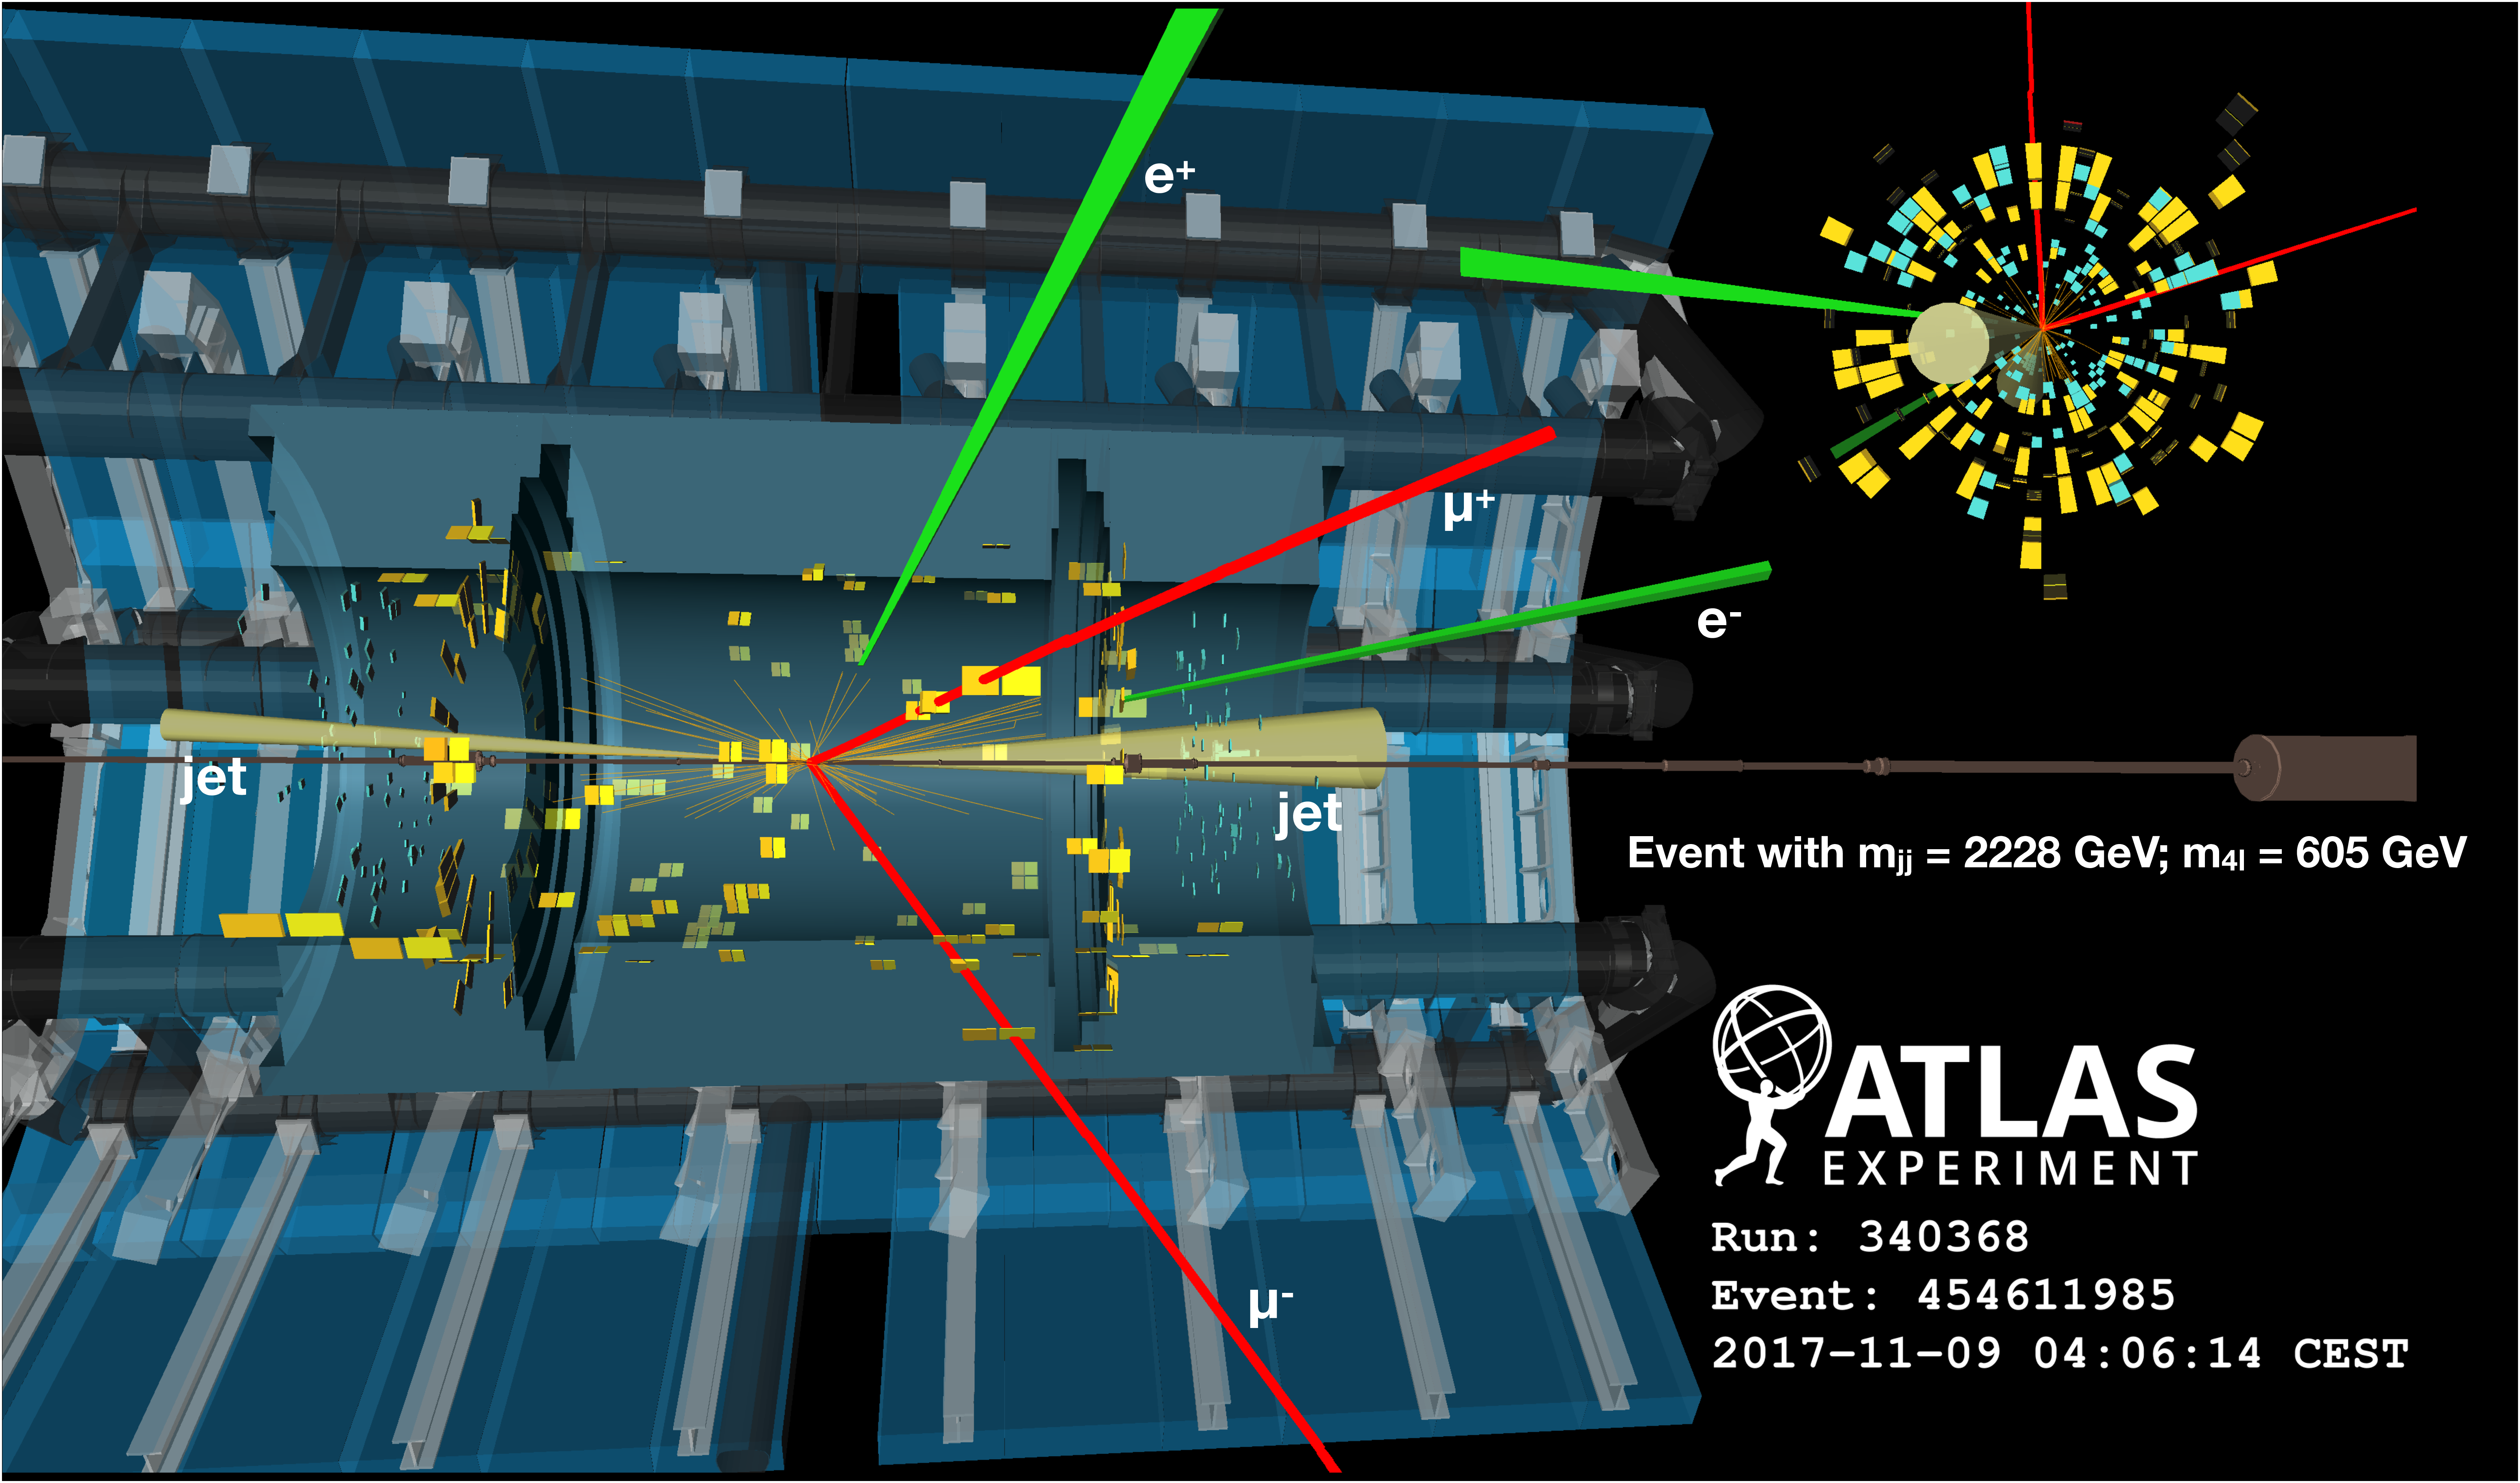
\includegraphics[width=.9\linewidth]{figures/AnalysisOverview/ZZjjEventDisplay.png}  
\caption{Event display of a candidate $pp \rightarrow ZZjj \rightarrow e^+e^-\mu^+\mu^- jj $ recorded by the ATLAS experiment in Run-$2$ $2017$ data-taking period. \label{fig:EventDisplayZZjj} \cite{ATLASZZjj}.}
\end{figure}